\documentclass[11pt, a4paper]{article}

% --- Packages ---
\usepackage[utf8]{inputenc}
\usepackage[T1]{fontenc}
\usepackage{mathptmx} % Times New Roman font for professional document typography
\usepackage{graphicx}
\usepackage[margin=0.8in]{geometry}
\usepackage{xcolor}
\usepackage{titlesec}
\usepackage{enumitem}
\usepackage{float}
\usepackage{booktabs}
\usepackage{multirow}
\usepackage{array}
\usepackage{url}

% Screenshots live in the repository's docs/images folder
\graphicspath{{../docs/images/}}

% --- Amrita Colors ---
\definecolor{amritaMaroon}{HTML}{A4123F}

% --- Title & Section Formatting ---
\titlespacing*{\section}{0pt}{12pt}{4pt}
\titlespacing*{\subsection}{0pt}{8pt}{3pt}
\titleformat{\section}{\large\bfseries\color{amritaMaroon}}{\thesection}{0.8em}{}
\titleformat{\subsection}{\normalsize\bfseries\color{amritaMaroon}}{\thesubsection}{0.6em}{}

\pagestyle{plain}

\begin{document}

% ==========================================
% HEADER & TITLE BLOCK
% ==========================================
\noindent
\begin{minipage}{\textwidth}
    \centering
    {\Large \textbf{\textcolor{amritaMaroon}{
    AMRITA VISHWA VIDYAPEETHAM \\
    SCHOOL OF COMPUTING \\
    DEPARTMENT OF COMPUTER SCIENCE AND ENGINEERING \\
    }}}
    \vspace{0.2cm}
    {\large \textbf{AranyaSetu: An FRA Spatial Intelligence and Decision Support Platform for Digitizing Legacy Forest Rights Records}} \\[0.1cm]
    \textbf{23CSE498 -- Project Phase II (External Review)} \quad | \quad \textbf{Team Number: [GXXX]} \\
    \today
\end{minipage}

\vspace{0.3cm}
\hrule
\vspace{0.3cm}

% --- Team & Guide Details ---
\noindent
\begin{center}
    \renewcommand{\arraystretch}{1.45}
    \setlength{\tabcolsep}{6pt}
    \begin{tabular}{|l|p{4.8cm}|p{4.6cm}|p{3.2cm}|}
        \hline
        \multicolumn{2}{|c|}{\textbf{Team Members}} & \textbf{Project Guide} & \textbf{Project Type} \\
        \hline
        \small [CB.SC.U4CSE23XXX] & \small \raggedright [Student Name 1] &
        \multirow{4}{=}{\raggedright \small \textbf{[Dr/Mr/Ms. Guide Name]} \newline \textit{[Designation], \newline Dept. of CSE}} &
        \multirow{4}{=}{\raggedright \small \textbf{Type 2} \newline Application-Based Project} \\ \cline{1-2}
        \small [CB.SC.U4CSE23XXX] & \small [Student Name 2] & & \\ \cline{1-2}
        \small [CB.SC.U4CSE23XXX] & \small [Student Name 3] & & \\ \cline{1-2}
        \small [CB.SC.U4CSE23XXX] & \small [Student Name 4] & & \\
        \hline
    \end{tabular}
\end{center}
\vspace{0.2cm}

\section{Abstract}
\noindent
Records of rights under the Forest Rights Act, 2006 \cite{fra2006} exist largely as scanned, handwritten or tabular legacy documents in Tamil and English, disconnected from any geographic reference. This makes it difficult for Gram Sabhas, sub-divisional and district-level committees, and revenue staff to verify claims, detect overlaps, or plan welfare schemes for forest-dwelling communities. This project presents \textit{AranyaSetu}, a web-based decision-support platform that follows the lifecycle \textit{Ingest $\rightarrow$ Structure $\rightarrow$ Spatialize $\rightarrow$ Enrich $\rightarrow$ Visualize $\rightarrow$ Recommend}. Scanned documents and CSV/XLSX registers are ingested into private storage after malware scanning, read with PaddleOCR \cite{du2020ppocr}, and converted into structured entities with field-level evidence, confidence and mandatory human review. Approved records are linked to native FRA claims, titles and versioned geometries stored in PostgreSQL/PostGIS \cite{postgis}. Bounded Sentinel-2 \cite{drusch2012sentinel2} acquisition and a pretrained Dynamic World \cite{brown2022dynamic} model supply land-cover evidence, which feeds an explainable rule-based scheme advisory engine. The system is implemented as a FastAPI \cite{fastapi} service with a separate durable-job worker, an OpenID Connect sign-in using PKCE \cite{rfc7636,oidccore}, an append-only audit trail, and a Leaflet-based Atlas interface. All modules are integrated into a working prototype. Verification comprised 521 passing backend tests, 93 passing browser-logic tests, nine passing real-browser workflow checks, and 263 passing PostgreSQL/PostGIS regression tests. The prototype uses synthetic data; it is not an adjudication system, and accuracy on real Tamil records has not been benchmarked.

% --- 2. PROBLEM DEFINITION & REQUIREMENT ANALYSIS ---
\section{Problem Definition \& Requirement Analysis}

\subsection{Problem Statement, Context \& Target Users}
\begin{itemize}[noitemsep, topsep=2pt]
    \item \textbf{Problem Definition:} Legacy FRA claim, verification and title records are held as scanned images, PDFs and spreadsheets without structured fields or geometry. Officials cannot search them by village or right type, cannot see claims on a map, cannot check whether claimed boundaries overlap, and cannot link a recognised right to the government schemes the holder may be eligible for.
    \item \textbf{Target Users \& Stakeholders:} Authorised staff (data-entry operators, reviewers, and officers at Gram Sabha, SDLC and DLC level) in Tamil Nadu, followed by individual claimants using a personal plot workflow and departmental scheme officers who receive referrals. Deployment is a server-hosted web application accessed from a standard browser.
    \item \textbf{Existing Limitations:} Generic OCR tools do not preserve page-level evidence, confidence and reviewer correction needed for legal records; ordinary cadastral (patta) tools treat land ownership and FRA rights as the same thing; and GIS tools lack claim workflow, audit and privacy controls \cite{fra2006,du2020ppocr}. Manual re-keying is slow and error-prone.
    \item \textbf{Application Objectives:}
    \begin{enumerate}[noitemsep, topsep=2pt]
        \item Convert scanned FRA documents and CSV/XLSX registers into reviewable structured records in which every approved value remains linked to its source page or row, extraction method and confidence.
        \item Spatialize claims and titles as versioned geometries, detect overlaps by right type, and display them in a synchronized, filterable Atlas.
        \item Enrich village records with reviewed satellite-derived land-cover observations and produce explainable, non-binding scheme recommendations with stated reasons and missing inputs.
        \item Protect private data through authenticated roles, private storage, malware scanning, rate limits and an append-only audit log.
    \end{enumerate}
\end{itemize}

\subsection{Functional \& Non-Functional Requirements}
\begin{table}[H]
    \centering
    \footnotesize
    \renewcommand{\arraystretch}{1.25}
    \begin{tabular}{|c|p{3.0cm}|p{9.2cm}|}
        \hline
        \textbf{Req. ID} & \textbf{Category} & \textbf{Requirement Specification} \\
        \hline
        FR-01 & Functional & Accept JPG, PNG, BMP, TIFF and PDF scans and UTF-8 CSV/XLSX registers; run OCR and extract Tamil and English FRA entities with evidence and confidence. \\
        \hline
        FR-02 & Functional & Provide reviewer correction and approval so that only approved values create or update native FRA claims, decisions and titles. \\
        \hline
        FR-03 & Functional & Import reference geometry (GeoJSON, zipped Shapefile, KML, GeoPackage), store versioned claim geometries, and evaluate overlaps by right type. \\
        \hline
        FR-04 & Functional & Acquire bounded Sentinel-2 scenes, run land-cover inference, and require staff review before observations enter the Atlas and DSS. \\
        \hline
        FR-05 & Functional & Return an explainable advisory scheme recommendation (outcome, reasons, missing inputs, model provenance) and allow a departmental referral. \\
        \hline
        NFR-01 & Non-Functional & Long-running OCR and imagery work must run as durable background jobs with renewable leases, bounded retry and quarantine, so API requests stay responsive. \\
        \hline
        NFR-02 & Non-Functional & Security and privacy: OIDC login with role-based access, malware scanning of uploads, private storage, shared request quotas, audit of sensitive reads, and no exposure of claimant identifiers or storage keys. \\
        \hline
        NFR-03 & Non-Functional & Reproducible deployment through Docker Compose and schema evolution through Alembic migrations, with PostgreSQL/PostGIS required in production. \\
        \hline
    \end{tabular}
    \caption{Summary of Application Functional and Non-Functional Requirements}
\end{table}

% --- 3. APPLICATION ARCHITECTURE & SOLUTION DESIGN ---
\section{Application Architecture \& Solution Design}

\subsection{End-to-End Application Architecture}
\noindent
A staff member signs in through the browser and the FastAPI service establishes a signed session. Uploaded documents are checked, scanned and written to private storage, then registered as durable jobs. A separate worker process leases each job, performs page-level OCR and entity extraction, and stores the results with the processed page image, so reviewers can compare each extracted field against the exact source pixels. After review, approved values create native FRA records, which are spatialized, enriched with satellite-derived observations, shown in the Atlas, and evaluated by the rule-based DSS. Every sensitive action is written to an append-only audit table.

\begin{figure}[H]
    \centering
    \small
    \fbox{\begin{minipage}{0.95\textwidth}
    \centering
    \vspace{3pt}
    \begin{tabular}{c}
    \textbf{Staff / claimant browser} (login, Archive, Cases, Atlas, DSS planner, personal plot portal) \\
    $\downarrow$ \\
    \textbf{FastAPI service} (OIDC session, rate limits, FRA / document / DSS / portal routes) \\
    $\downarrow$ \qquad\qquad\qquad $\downarrow$ \qquad\qquad\qquad $\downarrow$ \\
    \begin{tabular}{|c|c|c|}
    \hline
    Private storage \& ClamAV & Durable job queue $\rightarrow$ Worker & Redis (shared quotas) \\
    \hline
    \end{tabular} \\
    $\downarrow$ \\
    \begin{tabular}{|c|c|c|}
    \hline
    PaddleOCR + entity extraction & Sentinel-2 (STAC) + land-cover model & DSS rules + scheme catalogue \\
    \hline
    \end{tabular} \\
    $\downarrow$ \\
    \textbf{PostgreSQL / PostGIS} (claims, versioned geometry, evidence, observations, audit)
    \end{tabular}
    \vspace{3pt}
    \end{minipage}}
    \caption{End-to-End Application Architecture and Workflow}
\end{figure}

\subsection{Component Design, Data Flow \& Technology Stack}
\begin{itemize}[noitemsep, topsep=2pt]
    \item \textbf{Component Breakdown:} The \textit{API layer} (\texttt{app/api}) exposes FRA, document-intelligence, DSS and portal routes. The \textit{service layer} (\texttt{app/services}) contains intake, OCR, extraction, case, geospatial, satellite, asset, DSS, report, storage, malware, OIDC, OTP and audit logic. The \textit{worker} (\texttt{scripts.run\_fra\_jobs}) executes leased background jobs. The \textit{model gateway} keeps OCR, extraction and asset models behind replaceable, versioned adapters so trained models can be attached without changing the legal workflow.
    \item \textbf{User Interaction \& Interface Flow:} Sign-in leads to the FRA workspace with Archive review, native casework, geometry authoring, dashboards, Atlas and DSS planner. A separate user portal supports drawing and submitting a personal plot, which a staff member approves independently. Supporting cadastral evidence is a separate workspace and enters FRA casework only through reviewed legacy-intake controls.
    \item \textbf{Data Storage \& External Interfaces:} PostgreSQL 16 with PostGIS stores records and geometry through SQLAlchemy and Alembic (current migration head \texttt{20261114\_0019}); SQLite is supported for lightweight development. Original and derived artifacts reside on a private volume or Amazon S3. External interfaces are an OIDC identity provider, SMTP and Twilio for OTP delivery, a STAC imagery service, ClamAV and Redis.
    \item \textbf{Technology \& Deployment Stack:} FastAPI and Uvicorn; PaddleOCR/PaddlePaddle; OpenCV, Pillow and PDFium; Shapely, GeoAlchemy2, Fiona, Rasterio and PyProj; Leaflet for the browser map; Docker Compose services for API, worker, PostGIS, Redis and ClamAV.
\end{itemize}

% --- 4. COMPLETE IMPLEMENTATION DETAILS (100%) ---
\section{Implementation Details}

\subsection{Development \& Deployment Environment}
\begin{itemize}[noitemsep, topsep=2pt]
    \item \textbf{Platform \& Runtime Environment:} Python 3.11 on Linux containers for deployment; development and verification on Windows 11 with a Python virtual environment. Browser clients need no installation. Node.js 18 or newer is used only for browser-logic tests.
    \item \textbf{Libraries, Tools \& Hardware:} FastAPI 0.115, SQLAlchemy 2.0, Alembic, PaddleOCR 3.7 with PaddlePaddle 3.3, Shapely 2.1, Rasterio 1.4, Authlib, PyJWT, Redis client, boto3 and httpx; PyTorch CPU inference for the land-cover model; pytest, Node test runner and Playwright for testing. No special hardware is required; inference runs on CPU.
    \item \textbf{Source Code Repository:} \url{https://github.com/vTg2208/ocr-service} (branch \texttt{feature/open-source-model-integrations}), with operations, privacy, pilot and model-adapter documents under \texttt{docs/}.
\end{itemize}

\subsection{Module-Wise Implementation \& Integration Summary}
\begin{table}[H]
    \centering
    \footnotesize
    \renewcommand{\arraystretch}{1.25}
    \begin{tabular}{|p{3.5cm}|p{7.8cm}|c|}
        \hline
        \textbf{Application Module} & \textbf{Implemented Features \& Integration Details} & \textbf{Status} \\
        \hline
        Module 1: User Interface & Login, FRA Archive review, case management, Atlas, DSS planner, dashboards, printable privacy-safe reports, personal plot portal and cadastral evidence workspace. & 100\% (Integrated) \\
        \hline
        Module 2: Document Intelligence & Secure upload, malware scan, PaddleOCR, Tamil/English entity extraction, CSV/XLSX register import, field-level evidence with saved page overlays and reviewer approval. & 100\% (Integrated) \\
        \hline
        Module 3: Spatial \& Data Layer & PostGIS-backed claims, titles, versioned geometry, staged reference-vector import, overlap evaluation by right type, append-only audit, Alembic migrations. & 100\% (Integrated) \\
        \hline
        Module 4: Satellite \& DSS & Bounded Sentinel-2 acquisition, Dynamic World inference with SCL cloud masking, staff review, asset facts, explainable rule engine and departmental referrals. & 100\% (Functional) \\
        \hline
        Module 5: Security \& Operations & OIDC with PKCE, role-based access, Redis shared quotas, SMTP/Twilio OTP, durable job worker with leases and retry, Docker Compose stack. & 100\% (Functional)$^{*}$ \\
        \hline
    \end{tabular}
    \caption{Application Module Implementation and Integration Status. $^{*}$Provider adapters are implemented; live provider delivery and the Docker image build are not yet exercised (see Section~7).}
\end{table}

\subsection{Detailed Module Descriptions}
\begin{itemize}[noitemsep, topsep=2pt]
    \item \textbf{Document Intelligence:} Uploaded files are validated by type, scanned, stored privately, and enqueued. The worker renders PDF pages, preprocesses the image, runs PaddleOCR, and extracts entities (claimant, village, survey reference, right type, area and similar fields). Each field retains its source page or row, extraction method, confidence, schema version and the processed page frame with its dimensions and checksum, so a reviewer overlay is tied to exact pixels. Reviewer corrections never overwrite the original extracted value.
    \item \textbf{Spatial Casework:} Approved records create or link native FRA claims, decisions and titles. Geometries are versioned rather than replaced. Reference vectors are imported in a staged area, validated for CRS and geometry, repaired or flagged for duplicates, and published only after review. Overlaps are computed in PostGIS with square-metre and percentage thresholds that ignore slivers, and conflicts return an HTTP~409 with an audit record.
    \item \textbf{Satellite Enrichment and DSS:} For an approved plot or boundary, the system discovers bounded scenes from an allow-listed STAC service, reads the nine required bands with the matching scene-classification mask, and runs a pinned pretrained Dynamic World model on CPU. Results are stored privately with provenance and become Atlas observations only after staff review. The rule engine consumes derived facts and returns an outcome, reasons and missing inputs, and never approves or sanctions a benefit.
    \item \textbf{Security \& Operations:} Login uses authorization code with S256 PKCE, state, nonce and signed ID-token verification against a fixed issuer and audience; provider role claims never grant application roles. Request quotas use atomic Redis counters shared across instances and fail closed. Email and SMS verification store only digests with expiry and retry limits.
    \item \textbf{End-to-End Integration:} The browser, API, worker, database, storage and external adapters are wired into a single application that follows the lifecycle in Section~3.1. A seeded synthetic Tamil Nadu archive and a Villupuram pilot script exercise every stage from intake to scheme convergence.
\end{itemize}

% --- 5. FUNCTIONAL TESTING & PROTOTYPE DEMONSTRATION ---
\section{Functional Testing \& Prototype Demonstration}

\subsection{Functional Test Cases \& Verification}
\noindent
Verification combines automated suites with a real-browser run. The cases below summarize scenario groups covered by those suites; exact assertions are in the \texttt{tests/} directory.

\begin{table}[H]
    \centering
    \footnotesize
    \renewcommand{\arraystretch}{1.25}
    \begin{tabular}{|c|p{3.2cm}|p{3.4cm}|p{4.0cm}|c|}
        \hline
        \textbf{Test ID} & \textbf{Feature / Scenario} & \textbf{Input / User Action} & \textbf{Observed Output} & \textbf{Result} \\
        \hline
        TC-01 & Primary flow: legacy intake to review & Upload scan or register, run extraction, approve fields & Structured record with source evidence linked to approved values & Pass \\
        \hline
        TC-02 & Evidence overlays & Open a processed OCR page in review & Stored pixels match preprocessing; tampered artifact rejected & Pass \\
        \hline
        TC-03 & Module integration: geometry and Atlas & Publish geometry, filter Atlas & Claims and assets rendered consistently with list view & Pass \\
        \hline
        TC-04 & Boundary: competing parcel claim & Two requests claim same parcel & One accepted; other returns 409 and audit event & Pass \\
        \hline
        TC-05 & Satellite inference & Run analysis on Sentinel-2 input & Result stored privately with provenance; awaits staff review & Pass \\
        \hline
        TC-06 & Security: OIDC and quotas & Signed ID token; repeated requests across two instances & Valid login only; shared quota enforced & Pass \\
        \hline
        TC-07 & Evaluation integrity & Mix real and mock evaluation data & Mixed evaluation rejected; mock metrics flagged non-benchmark & Pass \\
        \hline
    \end{tabular}
    \caption{Functional Testing Summary Across Core Application Scenarios}
\end{table}

\noindent
\textbf{Automated results:} 521 backend tests passed (15 service-dependent tests skipped); 93 browser-logic tests passed; a native PostgreSQL~16/PostGIS~3.7 run passed 263 spatial, concurrency, worker, Atlas and DSS regression tests together with Alembic schema-drift checks; and a Playwright validation passed nine workflow and rendering checks with no JavaScript errors. Provider transports in OIDC, SMTP and Twilio tests are mocked at the protocol level.

\subsection{Working Prototype Demonstration}
\begin{figure}[H]
    \centering
    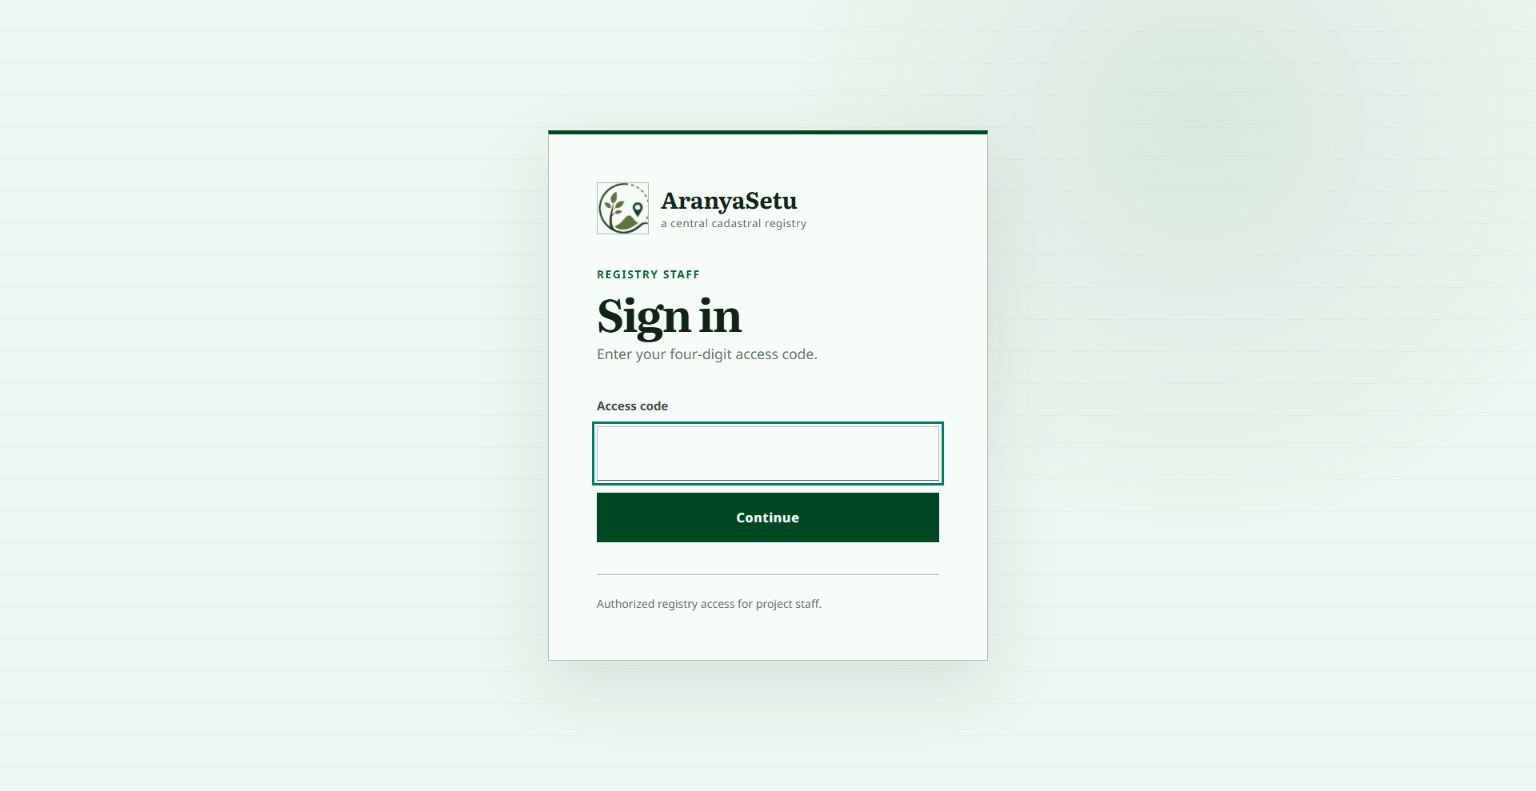
\includegraphics[width=0.46\textwidth]{aranyasetu-login.png}\hfill
    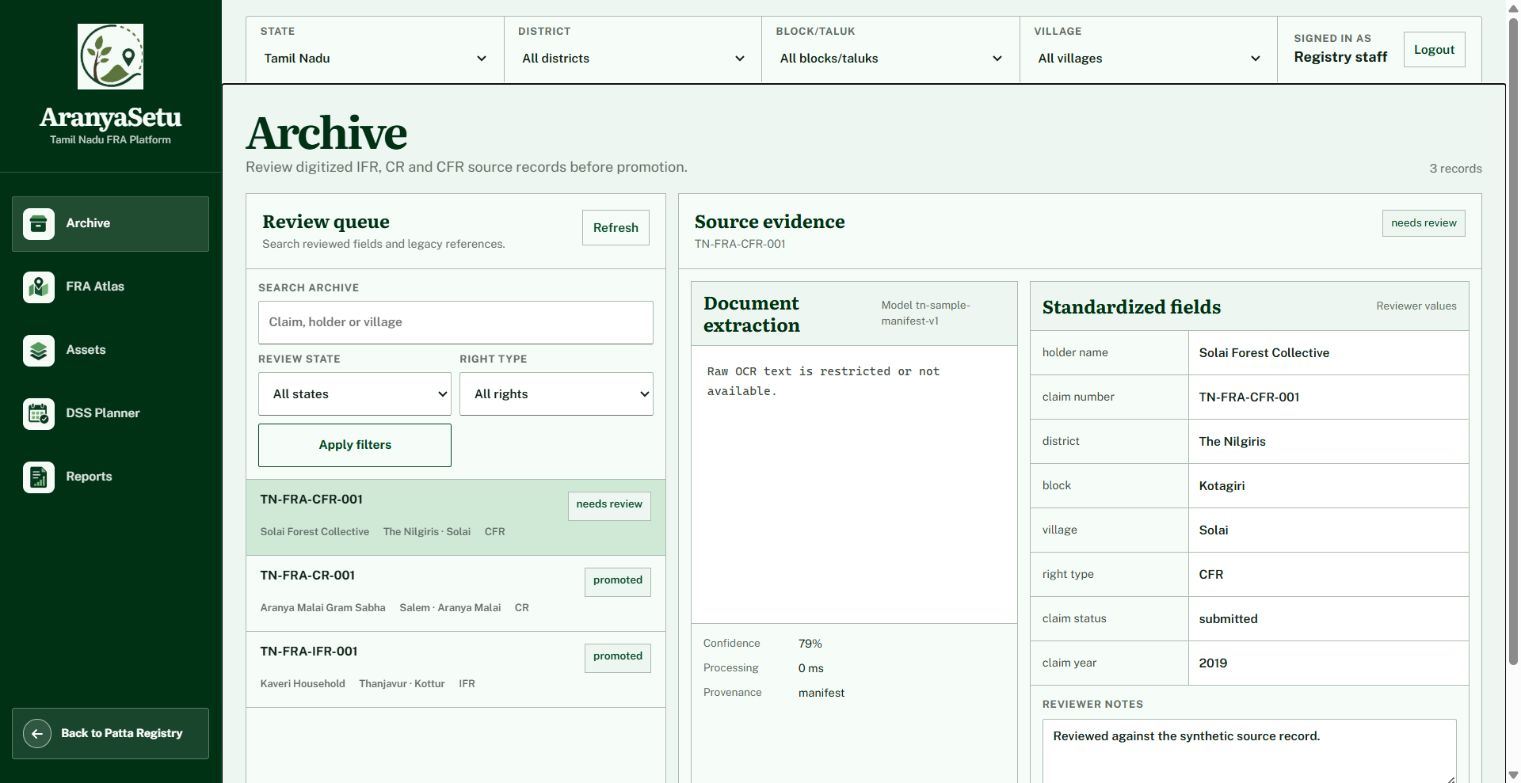
\includegraphics[width=0.46\textwidth]{aranyasetu-fra-archive.png}\\[4pt]
    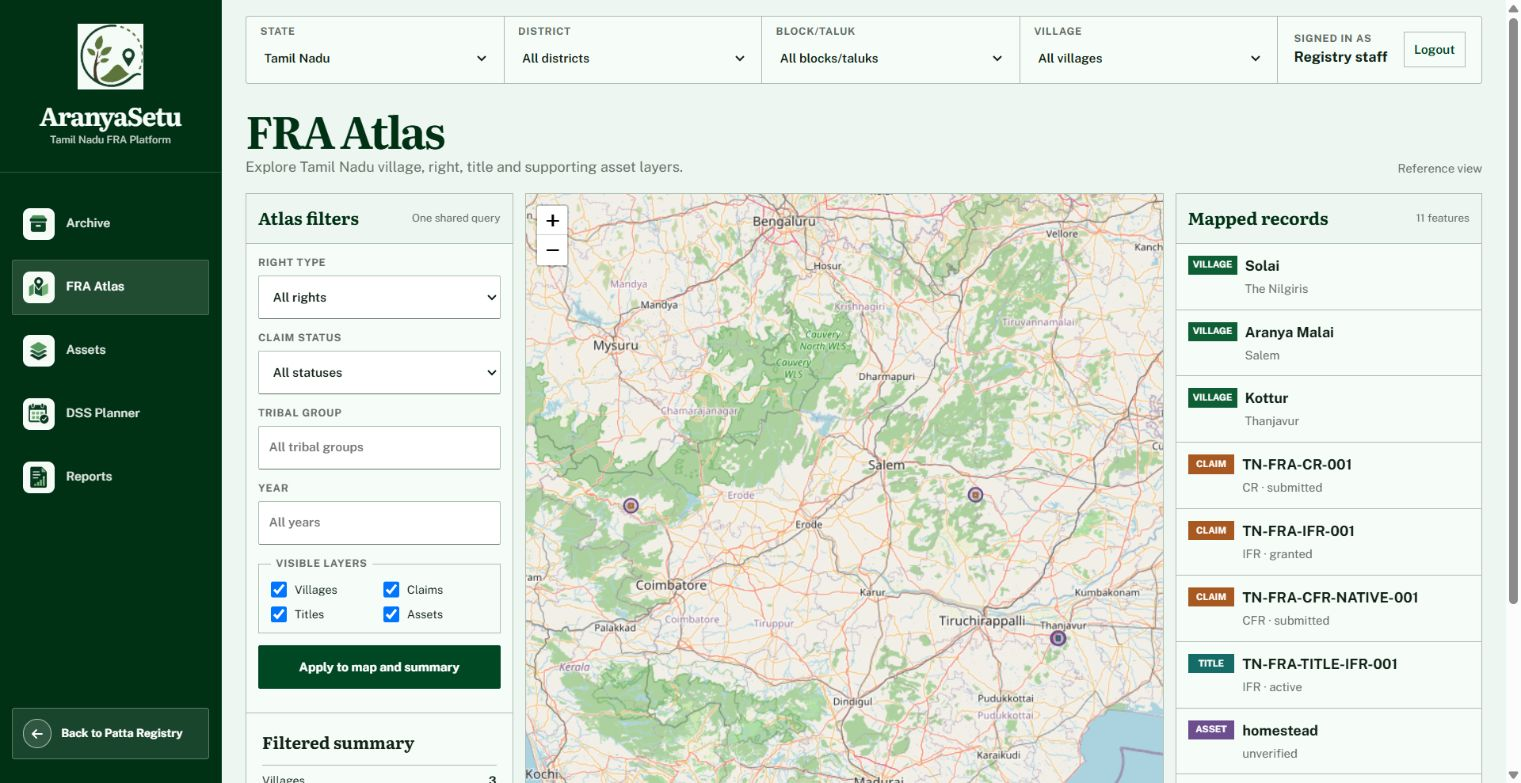
\includegraphics[width=0.46\textwidth]{aranyasetu-fra-atlas.png}\hfill
    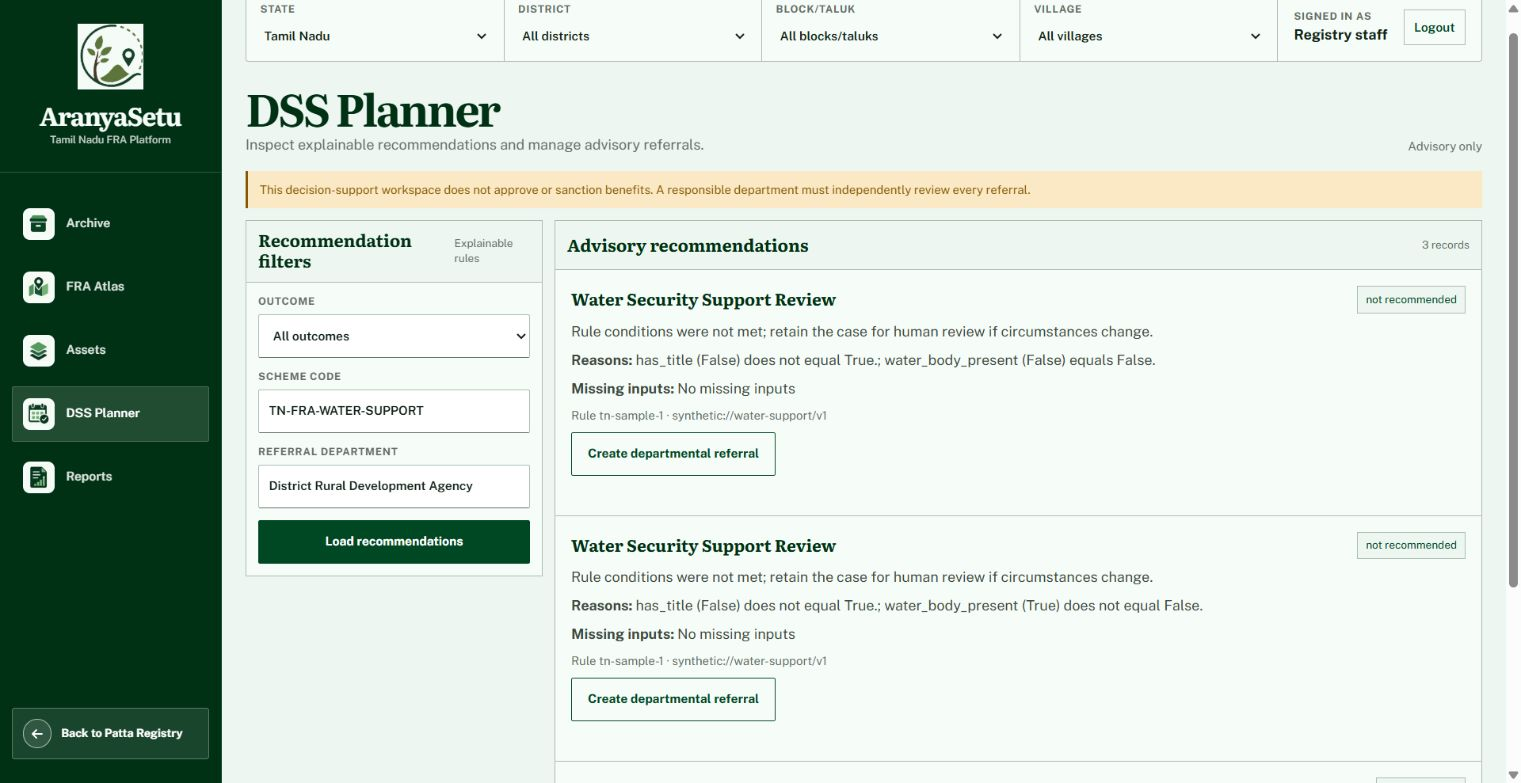
\includegraphics[width=0.46\textwidth]{aranyasetu-dss-planner.png}
    \caption{Working prototype using synthetic data: staff sign-in, Archive review, FRA Atlas, and explainable DSS planner.}
\end{figure}

\noindent
\textbf{Evaluation \& Usability Summary:} The prototype completes the intake-to-recommendation workflow on synthetic Tamil Nadu data in the browser. An actual PaddleOCR inference run recognised two lines of a generated English mock document after the official Tamil mobile detection and recognition models downloaded and initialised; this is an execution smoke check, not a Tamil OCR accuracy benchmark. Live Sentinel-2 execution succeeded, with no claim of local ground-truth accuracy. No user study has been conducted.

% --- 6. TECHNICAL KNOWLEDGE & ARCHITECTURAL DECISIONS ---
\section{Technical Justification \& Architectural Decisions}
\begin{itemize}[noitemsep, topsep=2pt]
    \item \textbf{Technology Stack Rationale:} FastAPI gives typed, documented APIs with low overhead \cite{fastapi}. PostGIS provides transactional spatial predicates and area computation needed for overlap detection \cite{postgis}. PaddleOCR offers open, Tamil-capable detection and recognition models \cite{du2020ppocr}. Dynamic World is an open pretrained land-cover model for Sentinel-2 \cite{brown2022dynamic}, avoiding the need for labelled training data the project does not have.
    \item \textbf{Architectural \& Performance Trade-offs:} OCR and imagery are slow, so they run in a separate worker with leases and bounded retry instead of inside request handlers, trading immediate results for responsiveness and recoverability. Model access sits behind versioned adapters, favouring modularity over a tightly coupled pipeline. CPU-only inference lowers cost and eases deployment at the expense of throughput. SQLite is kept for development, but production requires PostGIS because concurrency and spatial behaviour differ.
    \item \textbf{Security, Safety \& Error Handling:} OIDC with PKCE and fixed issuer and audience \cite{rfc7636,oidccore}; role-based access with operator-provisioned identities; upload type validation and ClamAV scanning; private, audited access to source documents; digest-only OTP storage; fail-closed quotas; human review before any extracted, spatial or satellite result becomes authoritative; and an append-only audit trail. Interrupted jobs are recovered, retried with backoff and finally quarantined for reviewer action. The DSS is advisory and never presented as legal adjudication.
\end{itemize}

% --- 7. CONCLUSION, LIMITATIONS & FUTURE SCOPE ---
\section{Conclusion, Limitations \& Future Scope}
\begin{itemize}[noitemsep, topsep=2pt]
    \item \textbf{Conclusion:} AranyaSetu delivers an integrated, reviewable pipeline from legacy FRA documents to spatial records, satellite-derived evidence and explainable scheme advice. It meets the stated functional and non-functional requirements as a testable prototype, with human review and provenance retained at every step.
    \item \textbf{Current Operational Limitations:} Bundled data is synthetic and the cadastral parcels are mock boundaries, not authoritative. Tamil OCR accuracy and land-cover accuracy have not been measured against verified labels. Live OIDC, SMTP and Twilio delivery, HTTPS hosting, backup and restore have not been validated with real provider credentials. The Docker images and full Compose stack were not built or run on the development machine, which has no Docker engine; native PostgreSQL/PostGIS verification was used instead. The system is a research prototype and not a legal land-ownership or FRA adjudication tool.
    \item \textbf{Future Enhancements:} Evaluate OCR and land-cover accuracy on verified Tamil labels and held-out land-cover data; attach trained models through the adapter gateway; import a licensed authoritative cadastral source; run the Compose release on a Docker host and complete production provider validation; and extend to further states and scheme catalogues.
\end{itemize}

% --- 8. DELIVERABLES & TECHNICAL ENRICHMENT SUMMARY ---
\section{Project Deliverables \& Technical Enrichment Summary}
\begin{table}[H]
    \centering
    \footnotesize
    \renewcommand{\arraystretch}{1.2}
    \begin{tabular}{|p{4.2cm}|p{7.5cm}|c|}
        \hline
        \textbf{Deliverable Category} & \textbf{Details / Title / Repository Link} & \textbf{Status} \\
        \hline
        Source Code Repository & \url{https://github.com/vTg2208/ocr-service}; README, operations, privacy, pilot and model-adapter documentation included & Completed \\
        \hline
        Individual Online Certifications & [List completed 10--20 hr courses for each team member] & [Completed] \\
        \hline
        Group TEA Deliverable 1 & [Title and details of completed Group Activity 1] & [Completed] \\
        \hline
        Group TEA Deliverable 2 & [Title and details of completed Group Activity 2] & [Completed] \\
        \hline
        Group TEA Deliverable 3 & [Title and details of completed Group Activity 3] & [Completed] \\
        \hline
    \end{tabular}
    \caption{Summary of Completed Project and Technical Enrichment Deliverables}
\end{table}

% --- REFERENCES ---
\vspace{0.2cm}
\nocite{*}
\renewcommand{\refname}{\large\bfseries\color{amritaMaroon}References}
\bibliographystyle{ieeetr}
\bibliography{ref}

\end{document}
